% !TeX program  = XeLaTeX
% !TeX encoding = UTF-8
\documentclass[a4paper]{nuist}
\usepackage{tikz}
\usetikzlibrary{plotmarks}
\usepackage{pgfplots}
\title{综述论文报告}
\author{
    周肖桐 \\
}
\date{\today}
\begin{document}

\maketitle
\newpage
\tableofcontents
\newpage

% \begin{equation}
%   \begin{aligned}
%       P_\theta(x_i)\\
%       x_1,x_2, \cdots, x_n\\
%       \vec{\theta}\\
%       \prod_{i=1}^{n} P_\theta (x_i)\\
%       \vec{\theta^*} =  \text{avg} \max \prod_{i=1}^{n} P_\theta (x_i)
%   \end{aligned}
% \end{equation}

% \begin{tikzpicture}
%   \begin{axis}[
%     xlabel=$x$,
%     ylabel=$P(x)$,
%     domain=-3:3,
%     samples=100,
%     smooth,
%     no markers,
%     axis lines=center,
%     x axis line style={->},
%     y axis line style={-},
%     ]

%     \addplot {exp(-x^2/2)/sqrt(2*pi)};

%     % 画两条竖线
%     \draw[dashed] (axis cs: 0, 0) -- (axis cs: 0, {exp(0)/sqrt(2*pi)});
%     \draw[dashed] (axis cs: 1, 0) -- (axis cs: 1, {exp(-1)/sqrt(2*pi)});

%     % 在两条竖线之间添加阴影
%     \fill[gray!20, domain=0:1]
%     (axis cs: -0.2, 0.5) -- % 使用 exp(0) 代替 exp(-0^2/2),即 x=0 处的值
%     (axis cs: -0.2, 0) -- (axis cs: 0.2, 0) -- (axis cs: 0.2, 0.5) -- cycle;

%   \end{axis}
% \end{tikzpicture}

% \begin{tikzpicture}
%   \begin{axis}[
%     xlabel=$x$,
%     ylabel=$P(x)$,
%     domain=-4:4,
%     samples=100,
%     smooth,
%     no markers,
%     axis lines=center,
%     x axis line style={->},
%     y axis line style={->}
%     ]
    
    
  
%     \addplot[fill=gray!20, draw=none, domain=-0.2:0.2, samples=50] {exp(-x^2/2)/sqrt(2*pi)} \closedcycle;
  
%   % 画两条竖线
%       \draw[dashed] (axis cs: -0.2, -0.1) -- (axis cs: -0.2, {exp(-0.04)/sqrt(2*pi)});
%       \draw[dashed] (axis cs: 0.2, -0.1) -- (axis cs: 0.2, {exp(-0.04)/sqrt(2*pi)});
%       \addplot {exp(-x^2/2)/sqrt(2*pi)};
%       \node at (axis cs: -0.52, 0.018) {$x_2$};
%       \node at (axis cs: 0.52, 0.018) {$x_2$};
%     \end{axis}
% \end{tikzpicture}


%\newpage

\section*{摘要}

本文介绍了风格迁移的由来以及分类。
\section{简介}

风格迁移是一种计算机视觉和图像处理领域的技术,它旨在将一幅图像的艺术风格应用于另一幅图像,从而创造出全新的图像。这一技术的应用非常广泛,从艺术创作到图像编辑都有涉及。风格迁移有两种主要方法:传统方法和基于神经网络的方法。

传统方法通常使用数学和信号处理技术,如纹理合成、直方图匹配和滤波等。这些方法涉及对图像的像素进行操作,以模拟所需的风格。例如,可以通过频域滤波来增强或减弱图像的某些频率成分,从而改变其外观。传统方法的好处在于它们通常计算速度较快,但它们可能无法捕捉到更高级的艺术风格和纹理。

基于神经网络的风格迁移方法则更加先进和强大。这些方法使用深度学习技术,来学习和应用图像的风格。它们通过训练神经网络来捕捉不同艺术风格的特征,然后将这些特征应用于输入图像,以生成具有所需风格的新图像。这种方法的好处在于它能够更好地捕捉到艺术风格的细节和复杂性,计算成本随使用的模型的差别而有所差别。

传统的风格迁移方法与基于神经网络的风格迁移方法之间并不应该事被代替与代替的关系,相反,目前许多基于神经网络的风格迁移方法的思想来源于传统的风格迁移方法。同时,基于神经网络的风格迁移技术也有一些缺陷,如伪影、难以控制风格化过程等缺陷,将传统风格迁移与基于神经网络的风格迁移工作相结合反而可能会取得更好的结果。

风格迁移技术的应用领域广泛,包括图像风格化、电影特效、艺术创作和图像编辑。无论是传统方法还是基于神经网络的方法,风格迁移都为图像处理提供了强大的工具,可以创建出富有艺术感和创新性的图像。

\section{传统风格迁移技术}

在神经网络兴起、风格迁移出现以前,就有类似的技术实现对艺术图像的模拟,非真实感绘制(Non-Photorealistic Rendering,NPR)与纹理模拟(Stroke-Based Rendering)是其中两种被广泛研究的技术。

%这一段是抄的,如果要发表需要重新组织
自20世纪90年代中期以来,艺术作品背后的艺术理论不仅吸引了艺术家,也吸引了许多计算机科学研究人员的关注。有大量研究和技术探索如何将图像自动转换为合成艺术品。在这些研究中,非真实感绘制(NPR)的取得了较大进展,如今它已成为计算机图形学界一个牢固确立的领域。然而,大多数 NPR 风格化算法都是针对特定的艺术风格设计的,并且不能轻易扩展到其他风格。在计算机视觉领域,风格迁移通常被研究为纹理合成的广义问题,即将纹理从源提取并迁移到目标。 \cite{QianWenHuaFeiZhenShiGanHuiZhiJiShuYanJiuXianZhuangYuZhanWang2020}

%这一段是抄的,如果要发表需要重新组织
NPR技术在发展过程中,研究者从图像建模的角度出发,基于笔触渲染、图像类比、图像 滤波的方法,对水彩画、素描画、油画等大众喜闻乐 见的艺术作品,水墨画、中国书法等来自中国的艺术 作品,以及蜡染画、版画等少数民族的艺术作品进行 数字化模拟研究,产生了大量优秀的艺术风格数字 化模拟作品,并成功应用于动画、遗产保护等领域。NPR 可对特定艺术风格,如水彩画、油墨画以及中国风的古 典画等各种画风进行数字化模拟。根据渲染方式不同, NPR 可细分为三类:笔触渲染、图像类比和图像滤波。 Meier\cite{meierPainterlyRenderingAnimation1996}提出基于笔触渲染的画笔模型,可以模拟油画生成的过程;Hertzmann 等人\cite{hertzmannImageAnalogies2023}提出图像类比的概念,在有监督的状态下改变原图风格;Winnemöller等人\cite{winnemollerRealtimeVideoAbstraction2006}引入双边滤波器和高斯差分滤波器来自动生成卡通风格图像。 纹理迁移技术主要用于纹理合成,即根据参考图像来对输入图像进行纹理填充,使得生成图像具有类似于样图的纹理风格,适用于处理纹理简单且重复的图像, 如木纹、砖块和墙面等。Efros 和 Leung\cite{efrosTextureSynthesisNonparametric1999}采用马尔科夫随机场(Markov Random Field,MRF)模型,选取与待填充像素点的邻域最接近的纹理片段来对该点进行像 素填充。这是早期纹理合成的经典算法,但该方法每填充一个像素值就需要遍历一次纹理片段,时间成本很高。\cite{TangRenWeiShenJingFengGeQianYiMoXingZongShu2021}

上述传统的风格迁移具有相同的缺陷,如仅考虑了图像的低层语义信息,而忽略了其高级语义信息、生成的纹理变化较少等。

\section{神经风格迁移技术}

随着神经网络的兴起,基于神经网络的风格迁移技术成为了该方向中较为主流的方法,本文称这种基于神经网络与深度学习的风格迁移技术为“神经风格迁移技术”。
为了能更好的介绍神经风格迁移技术,本文按迭代对象将神经风格迁移技术分为两类:基于像素迭代的风格迁移技术与基于模型迭代的风格迁移技术。前者的主要思想是利用损失函数对一张噪声图片进行迭代,从而得到一张风格化后的图像;后者对神经网络进行迭代,将风格图像的风格信息保存在神经网络的参数中,使该网络具有对特定的一种或多种风格进行迁移的能力。

以上两种迭代方法均有其子分类,且分类标准不同。对于“基于像素迭代的风格迁移技术”而言,可以根据使用的损失函数的类型进一步将其分类两类:基于格拉姆(Gram)矩阵的风格迁移技术与基于最大均值差(Maximum Mean Discrepancy,MMD)的风格迁移技术。%如图中所示〔此处需要插入图片:风格迁移技术的分类〕

对于“基于模型迭代的风格迁移技术”而言, 可以根据网络与网络所能进行转移的风格的数量进行分类,从而得到三个子类:一个风格对应一个网络模型,多个风格对应一个网络模型,任意风格对应一个网络模型。%如图中所示。〔此处需要插入图片:风格迁移技术的分类〕

本节以上述标准为主要行文思路,逐个对神经风格的代表性成果进行介绍。

\subsection{基于像素迭代的风格迁移技术}

DeepDream\cite{mordvintsevInceptionismGoingDeeper2015}第一个将卷积神经网络(Convolutional Neural Networks,CNN)提取出的结果进行反向重建,从而试图得到一张具有艺术风格的图像\cite{jingNeuralStyleTransfer2020},通过这种方式,DeepGream将深度学习与图像生成结合起来,这种“利用神经网络进行特征提取,再使用其他方法进行”为后来利用神经网络进行风格迁移打下了一定的基础。

在DeepDream之后,Gatys等人\cite{gatysImageStyleTransfer2016}于2016年再次将深度学习与风格迁移相结合,作出了突破性的成果,风格迁移的效果达到了一个新的高度%〔此处需要插入图片:Gatys等人风格迁移的成果〕。
在这之后,神经风格迁移的研究数量逐渐增长,目前正蓬勃发展。


\subsubsection{以Gram矩阵及其变体作为损失函数}

Gatys等人在于2016年发表的文献\cite{gatysImageStyleTransfer2016}中,将CNN与风格迁移结合,其主要工作可以分为两个部分:基于CNN的参数化纹理模拟以及基于反衍的图像重建过程\cite{gatysImageStyleTransfer2016}。基于CNN的参数化纹理模拟的思想来自于Gatys等人的一个发现,即一个使用足够数据训练的CNN可以提取进行跨数据集的图像特征提取\cite{gatysImageStyleTransfer2016}。在风格迁移领域中,对于一张照片而言,一个预训练的CNN网络能够提取其中的内容信息;对于一张具有特定风格的艺术图像,该CNN能够提取其中的风格信息。Gatys等人以此发现为基础,提出了一种基于像素迭代的风格迁移方法:定义一个损失函数,该损失函数以内容图像的高层特征与正在进行风格化的图像的高层特征之间的差异、以及风格图像与正在风格化的图像的高层特征之间的差异为主要内容。在该损失函数的指导下,将一张噪声图像认定为正在风格化的图像,对该噪声图像进行优化,直到损失函数达到最小值,以获得最终的风格化图像。损失函数的具体形式如下所示:
\begin{equation}
    \label{Gatys_total_loss}
    L_{total}=\alpha L_{content}+ \beta L_{style}
\end{equation}
其中,$L_{total}$是总体的损失函数,$L_{content}$是内容损失,代表正在风格化的图像与内容图像之间的内容差异程度,$L_{style}$是风格损失,代表正在风格化的图像与风格图像之间的风格差异程度,$\alpha$和$\beta$是超参数,用于控制生成的风格化图像与内容图像、风格图像之间的相似程度。

具体来说,内容损失函数$L_{content}$可以写成如下形式:
\begin{equation}
    L_{content}\left(\vec{p},\vec{x},l\right)=\frac{1}{2} \sum_{i,j} \left(F_{ij}^l-P_{ij}^l\right)^2
\end{equation}
其中,$\vec{p}$是输入的内容图像的展开,以向量的形式输入网络;$\vec{x}$是正在风格化的图像,同样的,需要对其进行展开成响亮的处理;$l$代表网络中的第$l$层,$F^l$为正在进行风格迁移的图像经过网络中第$l$层所生成的所有特征图的集合,$F_{ij}^l$表示上述风格化中的图像在神经网络第$l$层生成的特征图集合$F^l$的第$i$个特征图的展开向量中位于$j$位置的值;同理,$P^l$指的是输入网络的内容图像经过神经网络中的第$l$层处理后生成的所有内容特征图的集合,$P_{ij}^l$为上述内容特征图集合中的第$i$张内容特征图的展开向量中位于$j$位置的值。上述公式的含义在于逐像素计算风格化中的图像的特征图与内容图像的对应的特征图的差值并求和,利用梯度下降等方式对齐进行处理,使其最终稳定在一个较小的值,此时视为优化成功。

另一方面,在给出风格迁移函数$L_{style}$的具体表达式之前,需要首先介绍其核心——Gram矩阵。为了提取输入图像的风格特征,Gatys等人\cite{gatysImageStyleTransfer2016}使用了一个旨在捕获纹理信息的特征空间,该特征空间可以建立在网络任意卷积层的输出之上。该特征空间有不同卷积层的特征图之间的相关性构成,而上述相关性用第$l$层中第$i$张以及第$j$张向量化的特征图的内积表示,该内积就是Gram矩阵,记作$G^i \in R^{N_l\times N_l}$,Gram矩阵有公式如下:
\begin{equation}
    G_{ij}^l=\sum_k F_{ik}^lF_{jk}^L
\end{equation}

在此基础上,Gatys等人通过利用梯度下降对噪声图像进行处理,并以最小化原始图像的Gram矩阵与风格图像的Gram矩阵之间的均方距离为目标。网络中第$l$层在风格损失函数方面对$L_{style}$的贡献如下
\begin{equation}
    \label{Gatys_style_loss_l}
    E_l = \frac{1}{4N_l^2M_l^2}\sum_{ij}\left(G_{ij}^l-A_{ij}^l\right)^2
\end{equation}
其中,$N_l$为网络中一个卷积层中卷积核的个数,也即该层网络能够生成的特征图的个数,$M_l$是特征图包含的像素的个数,在数值上等于特征图的长度与宽度的乘积,$A_{ij}^l$和$G_{ij}^l$分别表示网络第$l$层中第$i$张向量化特征图上位于$j$位置的像素值。公式\ref{Gatys_style_loss_l}仅计算了网络单层对风格损失$L_{style}$的影响,将所有层中的损失带权相加即为$L_{style}$,其具体形式如下:
\begin{equation}
    L_{style}\left(\vec{a},\vec{x}\right)=\sum_{l=0}^L \omega_l E_l
\end{equation}  
其中,$w_l$是每一层对于总风格损失函数的影响权重,$L$为网络中卷积层的个数。将式\ref{Gatys_total_loss}进行偏导计算,得到结果$\frac{\partial L_{total}}{\partial \vec{x}}$,该结果可以作为作为优化算法的输入,并指导风格化中的图像进行迭代,以完成风格迁移的效果。

Gatys等人首创的以Gram矩阵为核心的风格迁移方法具有鲜明的优点。与以往的传统风格迁移方法相比,具有突破传统风格迁移效果笔触呆板、变化度少的优秀的效果;同时,突破了传统方法仅能对特定风格进行迁移的缺陷,实现了对自然的纹理以及风格化的纹理进行迁移\cite{jingNeuralStyleTransfer2020},从而获得良好的迁移效果。但是,此方法存在一些明显的缺陷。由于每次风格迁移都是从一张噪声图像开始,因此在批量进行风格迁移时,需要花费大量的时间,并在实时风格迁移方面效果较差。除此之外,Gram矩阵更擅长提取特征图的全局信息,这导致对具有长程对称结构的规则纹理的提取效果不能令人满意\cite{jingNeuralStyleTransfer2020}。同时,与传统风格迁移忽略高层语义信息不同的是,由于Gatys等人的方法仅仅考虑了图像中的高层语义信息,而忽略了其中的低层语义信息,导致了合成的风格化图像中精细结构与细节连贯性方面有所缺陷。

为了解决这个问题,Berger\cite{bergerIncorporatingLongrangeConsistency2016}等人对Gaty等人进行改进,提出了水平垂直像素差异,该方法计算了特征图中位于$(i,j)$位置的像素与位于$(i,j+\delta)$或位于$(i+\delta,j)$的像素之间特征关系,并将之纳入风格损失的考量。通过这种方式,能更有效的对具有对称性的长纹理图案进行迁移,从一定程度上弥补了Gatys等人对于精细结构与长程对称结构的规则纹理的模拟效果的不足。同时,由于使用了Gram矩阵作为风格迁移的核心,所以本方法依旧保留了一部分Gatys等人方法的缺陷,如对细节纹理的模拟不到位。

Risser\cite{risserStableControllableNeural2017}等人针对Gatys等人的方法进行研究,并发现了Gram矩阵用于风格迁移时不稳定的原因:具有不同均值和方差的特征图可能拥有相同的Gram矩阵。基于这个发现,Risser等人将特征图的直方图纳入风格迁移损失函数的考量,进一步优化了基于Gram矩阵的风格迁移方法。其优点在于能够生成更加稳定的风格图像;但由于引入了特征图的直方图,导致该方法的计算更加复杂,风格迁移过程耗时更长,在进行批量迁移时效率更低。同时,由于Risser等人仅考虑了风格化过程中生成图像的稳定性问题,不能对纹理精细化描述的问题依旧存在。

上述基于Gram矩阵的神经风格迁移效果存在一些共有的缺陷。由于卷积神经网络丢失了一些图像中的低层信息,导致对于具有规则形状的物体(如人工制造的物件)的迁移结果中往往存在一些不可忽视的扭曲现象。同时,风格化的过程会花费大量的时间,在对大量图像进行风格迁移时需要大量的时间,在诸如视频风格迁移等具有大量图像的任务中效率较低,且生成风格不稳定。

\subsubsection{以MMD及其变体作为损失函数}

Li等人\cite{liDemystifyingNeuralStyle2017}认为神经风格迁移任务可以视作领域自适应任务的一个特殊的变种任务,以此为切入点,Li等人得到了不一样的视角。领域自适应任务基于一个事实,即源数据与目标数据的分布不同,其目的是通过在一个带有标签的源域数据集上进行训练,以得到一个能够预测目标领域数据分布情况的模型。领域自适应任务的一种方法是通过最小化源域和目标域中样本的分布差异,从而实现源域与目标域中样本的匹配,其中最大均值差异(Maximum Mean Discrepancy,MMD)是度量两个域之间差异的常用选择。类比到风格迁移任务中,内容图像可以看作是该领域自适应的源域,而风格化的图像即是目标域。Li等人探究了Gram矩阵在风格迁移中的数学作用,证明了对风格图像与风格化中的图像的Gram矩阵的匹配过程,即公式\ref{Gatys_style_loss_l},本质上与最小化一个具有二次多项式核的MMD相同。因此,Li等人认为,最小化具有其他核函数(如线性核、多项式核、高斯核)的MMD可能会在风格迁移领域中具有一定的作用。Li等人的主要贡献在于从理论方面探寻并发现Gatys等人方法的原理,使其在原理方面更加清晰。

\subsubsection{基于马尔科夫随机场的神经风格迁移}

使用马尔科夫随机场(Markov Random Fields,MRF)进行纹理模拟是传统风格迁移领域中一个较为常见的方法\cite{ChenHongJiYuYangBenXueXiDeXiaoXiangHuaZiDongShengChengSuanFa2003,liMarkovRandomField1994,crossMarkovRandomField1983,chellappaTextureSynthesisCompression1985,bennettMultispectralRandomField1998},Li和Wand等人\cite{liCombiningMarkovRandom2016}将MRF与深度卷积神经网络(Deep Concolutional Neueal Networks,dCNN)相结合,提出了非参数化的神经风格风格迁移方法。他们认为,使用Gram矩阵的参数化风格迁移方法仅考虑了像素和像素之间的差异,没有从空间层次角度对风格化图像进行约束,从而导致了在生成的图像合理性不足。因此,Li和Wand等人将Gram矩阵替换为MRF正则化器,并引入了一个新的损失函数:
\begin{equation}
    L_s=\sum_{l\in {l_s}}\sum_{i=1}^m \mid\mid\Psi_i(F^l(I))-\Psi_{NN(i)}(F^l(I_s))\mid\mid^2
\end{equation}其中,$\Psi(F^l(I))$是特征图$F^(I)$所有局部块的集合;$\Psi_i(F^l(I))$为特征图所有局部块集合中的第$i$个;$\Psi_{NN(i)}$是风格化图像$I$中与第$i$个局部块风格最相似的风格块,可以通过计算风格图像中所有风格块的归一化关系从而得到上述最佳匹配的风格化块$\Psi_{NN(i)}$;$m$为局部块的总数。Li和Wand等人的方法增强了Gatys等人风格迁移的效果,使得风格化图像中物体的结构更具合理性,可以更好的保留原图的精细结构,并在合成真实照片方面取得了较大的进步。但同时,如果内容与风格图像在结构上存在较大差异时,局部块与风格块的匹配度可能不高,图像块无法正确匹配,最终导致该方法生成的风格图像的效果较差。


\subsubsection{基于Diffusion的风格迁移}

Diffusion模型是一种生成模型,最早由Ho等人\cite{hoDenoisingDiffusionProbabilistic2020}给出了详细的数学证明、推导与可运行的代码。Diffusion模型可以从噪声中生成目标数据样本。它包括两个过程:前向过程(forward process)和逆向过程(reverse process),其中前向过程又称为扩散过程(diffusion process)。前向过程是加噪的过程,前向过程中图像$ x_t $只和上一时刻的 $x_ {t-1}$ 有关, 该过程可以视为马尔科夫过程, 满足: 
\begin{equation}
    q (x_ {1:T}|x_0) = \prod_ {t = 1}^ {T}q (x_t|x_ {t-1}) q (x_t|x_ {t-1}) = N (x_t, \sqrt {1-\beta_t}x_ {t-1},\beta_t I)
\end{equation} 
其中不同t的 $\beta_t$ 是预先定义且逐渐衰减的,并满足 $\beta_1<\beta_2<...<\beta_T$。逆向过程是去噪的过程,如果得到逆向过程$ q (x_ {t-1}|x_ {t})$ ,就可以通过随机噪声 $x_T$ 逐步还原出一张图像。

Hamazaspyan与Navasardyan\cite{hamazaspyanDiffusionEnhancedPatchMatchFramework2023}将diffusion模型与风格迁移任务相结合,提出了扩散增强的块匹配(Diffusion-Enhanced PatchMatch,DEPM)模型。该模型利用Stable Diffusion来捕获高级风格特征,同时保留原始图像的细粒度纹理细节。DEPM允许在推理过程中转移任意样式,而无需任何微调或预训练,从而使过程更加灵活和高效。

Zhang等人\cite{zhangInversionBasedStyleTransfer2023}在Diffusion模型的基础上提出了具有全新思想的风格迁移——将学习各艺术风格中的隐含文字标签作为风格迁移核心。该方法的主要思想是将艺术画中的风格看作一幅画的可学习的文本描述,并根据风格标签指导Diffusion模型生成图像。在具体实现方面,Zhang等人利用所提出的反衍风格迁移方法(Inversion-Based Style Transfer Method,InST)高效准确的学习图像相关信息。具体来说,使用条件生成模型学习图像和文本之间的对应关系,从而获得图像嵌入;在图像嵌入的基础上,利用注意力导向的反转模块接收到图像嵌入,并利用注意力机制来生成对应的文本嵌入。该模块会关注图像嵌入中的不同特征,例如语义、材质、对象形状、笔触和颜色等,最终得到对应的文本嵌入,及文本标签。利用文本标签即可指导Diffusion模型进行风格迁移。该文本标签并不一定可以用自然语言描述出来,是一种只有Diffusion模型可以读懂的对风格进行描述的一串字符或者一个令牌(token)。该文本标签一经学习,Diffusion即可固定该标签对应风格,在这个层面上,可以视本方法为基于模型迭代的风格迁移方法。本文最大的特色是可以改变风格化过程中图像的形状,这是以往风格迁移模型所不能的。

Wang等人\cite{wangStyleDiffusionControllableDisentangled2023}利用Diffusion模型实现了图像风格与图像内容的分离。Wang等人构建了一种名为StyleDiffusion的框架,用于实现可控的分离风格转换。该框架基于Diffusion模型,通过扩散过程分别移除图像中的风格信息和内容信息,并通过协调样式重建先验的基于CLIP的样式解缠损失,实现了内容和风格的完全解缠。框架由三个关键组成部分:基于扩散的风格去除模块、基于扩散的风格转移模块以及与风格重建先验协调的基于CLIP的风格解缠损失。实验证明,该框架能够生成高质量的风格转换结果,并且相对于其他方法,更好地考虑了内容和风格之间的关系。与之前的方法相比,本文方法通过扩散模型完全解耦了内容(C)和风格(S),从而更好地考虑了它们之间的关系。这样一来,风格转换结果更加自然和和谐(尤其对于具有挑战性的风格,如立体派和油画)。Wang等人的方法通过扩散模型和基于CLIP的风格解耦损失,实现了对风格转换过程的精确控制。通过调整参数,可以灵活地控制风格去除的程度和内容与风格的解耦程度,从而得到更加理想的风格迁移效果。同时,该模式具有较高的可解释性和可扩展性。通过引入扩散模型和基于CLIP的风格解耦损失,风格迁移过程更具可解释性。此外,该方法还可以应用于其他图像转换或操作任务,具有一定的扩展性。

Lu等人\cite{luSpecialistDiffusionPlugandPlay2023}试图利用Diffusion模型解决如何通过少量图像样本对预训练的扩散模型进行微调,以学习任何未见过的风格的问题。Lu等人提出了一种名为"Specialist Diffusion"的方法,它可以通过对预训练的扩散模型进行微调来学习任何未见过的风格。通过仅使用少量图像(例如少于10张),便可以对预训练的扩散模型进行微调,使其能够以指定风格生成任意对象的高质量图像。为了实现这种极低样本微调,Lu等人提出了一套新颖的微调技术,包括文本到图像的定制数据增强、内容损失以促进内容和风格的解耦,以及只关注少数时间步骤的稀疏更新。"Specialist Diffusion"方法可以与现有的扩散模型和其他个性化技术无缝集成,并在学习高度复杂的风格时,以超级高效的微调效果胜过最新的少样本个性化扩散模型。此外,"Specialist Diffusion"可以与反转方法相结合,进一步提高性能,甚至在非常不寻常的风格上也能取得成功。但同时,该方法存在一定的局限性。首先,虽然本方法可以通过少量图像进行微调来学习未见过的风格,但是对于一些高度特定和不寻常的风格,仍然可能存在学习不充分的情况。其次,本方法在样本效率上取得了很好的效果,但对于某些复杂的或接近训练数据分布的内容,生成的结果可能不尽如人意。最后,本方法的性能受到预训练模型的限制,如果预训练模型的质量不高,可能会影响到微调后的结果。

由于卷积神经网络(CNNs)的局部性,提取和维护输入图像的全局信息变得困难,传统的神经风格迁移方法存在内容偏倚的问题。为了解决这个问题,Deng等人\cite{dengStyTr2ImageStyle2022}提出了一种基于Transformer的方法,称为StyTr2,该方法考虑了输入图像的长距离依赖关系。与其他视觉任务的视觉Transformer不同,StyTr2 包含两个不同的Transformer编码器,分别用于生成内容和风格的特定领域序列。在编码器之后,采用多层Transformer解码器根据风格序列对内容序列进行风格化。同时,Deng等人还分析了现有位置编码方法的不足,并提出了适用于图像风格迁移任务的内容感知位置编码(CAPE),它具有尺度不变性,更适合图像风格迁移任务。但是该方法存在一定的局限性。1. 对于与训练示例分辨率不同的输入,学习方法可能会出现垂直轨迹伪影的问题。2.传统的基于CNN的方法在重复迭代的过程中可能会导致生成的内容结构变得模糊,尽管该方法可以减轻这个问题,但仍存在一定程度的内容泄漏。3.本文中使用的Transformer架构相对于传统的CNN方法可能会增加计算复杂度,导致算法的运行时间较长。
\subsection{基于模型迭代的风格迁移技术}

基于像素迭代的风格迁移技术虽然取得了开创性的成果,但其中问题依然存在。在考虑将风格迁移方法进行应用时,一个较为明显的缺陷暴露出来,即迁移时间长,无法对进行实时的风格化操作,同时在进行大量特定风格的迁移任务时花费时间巨大,基于模型迭代的风格迁移技术的出现解决了对特定风格进行批量迁移的长耗时问题。按模型与其所能生成的风格数量的对应关系,可以将基于模型迭代的风格迁移技术分为三类:单模型生成单风格、单模型生成多风格以及单模型生成任意风格。

\subsubsection{单模型生成单风格}

Johnson等人\cite{johnsonPerceptualLossesRealTime2016b}与Ulyanov\cite{ulyanovTextureNetworksFeedforward2016b}等人于2016年彼此独立地提出了利用前馈神经网络进行实时风格迁移的想法,其主要思想是训练一个前馈神经网络
\begin{equation}
    \begin{aligned}
        \theta^* &= \arg\min L_{total}\left(I_c,I_s,g_\theta*(I_c)\right),\\
        I^*&=g_\theta*(I_c),
    \end{aligned}
\end{equation}
其中,$\theta^*$为最优的参数,即令损失函数$L_{total}$取最小值的参数;$L_{total}\left(I_c,I_s,g_\theta*(I_c)\right)$是整体的损失函数,它衡量了风格迁移的质量,该函数的输入包括三个部分,$l_c$表示内容图像,$l_s$表示风格图像,$g_\theta*(I_c)$表示对内容图像进行修改从而使其具有与风格图像相似外观的结果,即风格化中的图像;$I^*$是最终生成的图像,也就是风格迁移后所得的风格化图像。该公式的目标是找到一个能够最小化$L_{total}$的参数$\theta^*$,该参数被用于将内容图像$l_c$转换为最终的风格化图像$I^*$。Johnson等人与Ulyanov等人的区别仅在于二者的网络结构的差异:Johnson等人在Rardford等人\cite{radfordUnsupervisedRepresentationLearning2016a}方法的基础上,添加了残差块与分步卷积,并引入的实例归一化层( Instance Normalization,IN)以加快网络的收敛速度;Ulyanov等人以多尺度结构作为生成网络,目标函数与Gatys等人类似。Johnson等人与Ulyanov等人均以前馈生成网络为基础,达成了实时风格迁移的效果,风格迁移的速度Gatys等人相比,提升了两个数量级。但由于两人的方法遵循了Gatys等人提出方法,所以在迁移效果方面存在类似的问题,如在图像细节与结构合理性方面效果不能令人满意。

利用马尔科夫随机场也可以达成提升迁移速度的目的。Li和Wand等人\cite{liPrecomputedRealTimeTexture2016}在他们之间的工作\cite{liCombiningMarkovRandom2016}的基础上进行改进,他们通过对抗训练获得一个马尔科夫前馈网络,从而解决的效率问题。从原理上来说,该方法类似于他们之前在\cite{liCombiningMarkovRandom2016}中的方法,是一种基于图像块的非参数风格迁移方法,这使得他们的方法在物体结构的合理性方面具有更好的效果,从而更好地保留原图的精细结构。但同样的,该方法遗留了原始方法的一些缺点,如局部块与风格块的匹配度不高时,生成的风格图像效果较差。

利用生成式对抗网络(Generative Adversarial Networks,GAN)进行风格迁移也是一种基于模型迭代的风格迁移方法。GAN由Goodfellow等人\cite{goodfellowGenerativeAdversarialNetworks2020}于2014年提出,该模型采用一个生成网络和一个判别网络进行对抗。在训练时,需要先对判别网络进行训练:给定一组数据,判别网络判断该组数据中的每一个数据项是否属于目标域,并根据真实值与网络计算得到的判断值之间的差距进行优化,直到能够判断测试集中的数据项是否属于目标域:随后对生成器进行训练,生成器生成数据,交由判别器进行判断是否属于目标域,生成器再根据判别器给出的结果进行调整,生成器与判别器二者不断进行对抗,以达到两个网络之间的均衡,从而完成网络的训练,并实现生成数据与真实数据之间分布的相似。GAN的损失函数如下所示:
\begin{equation}
    V(D,G)=\mathbb{E}_{x\sim p_{\text{data}}(x)}\left[\log D(x)\right]+\mathbb{E}_{z\sim p_{\text{z}}(z)}\left[\log \left(1-D(G(z))\right)\right]
\end{equation}
其中,$G$与$D$分别为生成器网络与判别器网络,$p_{\text{data}}(x)$表示数据$x$所满足的分布,$ p_{\text{z}}(z)$表示噪声图像的分布,$D(x)$表示$x$属于真实数据而非输入生成器生成的数据$p_g$的概率,$G(z)$表示生成器对噪声图像的处理结果,$\mathbb E$表示期望。训练判别器的过程以最大化判别器能否识别来自数据集而非生成器$G$的图像的概率;生成器的训练过程以最小化$\log \left(1-D(G(z))\right)$为目标,$1-D(G(z))$表示判别器认为生成器生成的图像不属于真实数据集的概率,最小化该函数及欺骗判别器,使其认为生成器生成的数据来自真实数据集。

GAN模型优秀的网络结构使其能够胜任风格迁移的任务,以下是GoodFellow等人在文献\cite{goodfellowGenerativeAdversarialNets2014a}中给出的一些迁移例子%〔此处需要插入图片:Goodfellow等人的迁移图像〕。

GAN网络同样实现实时风格迁移,但同时存在一些问题与缺陷。首先,GAN的训练通常比较困难,容易出现训练不稳定的情况,如模式崩溃(mode collapse)等。其次,GAN模型的损失函数并未给出类似于Gatys等人\cite{gatysImageStyleTransfer2016}损失函数中的超参数$\alpha$与$\beta$,从而导致了无法控制生成图像与内容图像或风格图像的相似读,在风格迁移任务中难以细粒度地控制两者。

ZHU等人\cite{zhuUnpairedImageToImageTranslation2017a}提出的CycleGAN实现了无监督的风格迁移任务CycleGAN的独特之处在于它引入了“循环一致性损失”,并通过同时训练两个生成器与判别器实现该损失,从而确保了转换是双向的,即可以从一个域到另一个域,然后再返回,在此过程中不会丢失信息。与GAN类似,生成器旨在将图像从一个域映射到另一个域,判别器则试图区分生成的图像和真实图像。CycleGAN 的最大优势之一是其能够处理非配对数据从而实现无监督学习,该方法能够学习如何进行跨域图像转换,而无需在训练时提供每个样本的明确匹配。但同时,CycleGAN在风格迁移领域有一些明显的缺陷,其生成的图像有时可能比真实图像更模糊甚至失真。其次,选择不当的超参数可能导致训练过程不稳定,或者生成质量较差的图像。

\subsubsection{单模型对应多风格}

上述基于模型迭代的风格迁移方法虽然解决了实时风格化的问题,提升了风格迁移的效率,但是每个模型只能对应某个特定的风格,进行新风格的迁移时,需要花费大量的时间进行新模型的训练。利用网络中的参数共享可以很好的实现多风格迁移效果。

Dumoulin等人\cite{dumoulinLearnedRepresentationArtistic2017}等人提出了一种能够生成多种风格的迁移网络。Dumoulin等人认为,部分不同风格的迁移工作中存在相似或者相同的计算部分,因为许多名称不同的艺术风格具有相似或相同的笔触(如印象派绘画具有相似的笔触,区别仅在使用的画面中使用的颜色),将这些具有相似笔触的画作看成不同的风格似乎是很浪费的。而传统一对一的风格迁移模型忽略了这一点,导致在对新风格进行迁移时,造成了不必要的时间浪费。在如何将这个想法付诸实践的过程中,Dumoulin等人\cite{dumoulinLearnedRepresentationArtistic2017}发现,只需要将标准化后的参数进行缩放或者移动,就能适应每种特定的风格;对于一个卷积神经网络而言,这个发现表示网络中所有卷积核的参数可以在不同风格中进行共享。这个发现表明,在进行风格迁移时,只需要在归一化后对某些参数进行调整,即可实现利用对不同风格的迁移。从具体实现层面,Dumoulin等人\cite{dumoulinLearnedRepresentationArtistic2017}在Ulyanov等人\cite{ulyanovTextureNetworksFeedforward2016b}的方法的基础上,在进行实例归一化后继续进行了一次仿射变换,即可完成对不同风格的迁移工作。这个过程被他们乘坐条件归一化(Conditional Instance Normalization,CIN),可以用如下公式表示:
\begin{equation}
    \label{IN}
    IN(x)=\gamma \left(\frac{x-\mu(x)}{\sigma(x)}\right)+\beta
\end{equation}
公式中,$\mu(x)$与$\sigma(x)$分别表示图像的均值与标准差。该方法将每种风格与两个参数$\gamma$与$\beta$绑定,从而实现使用单个网络对不同的风格进行迁移的效果。

Chen等人\cite{chenStyleBankExplicitRepresentation2017a}的方法利用了解耦合的思想,即利用单独的网络组件来学习,从而实现了由多个卷积核组成的网络结构“StyleBank”。StyleBank中的每一组卷积核代表了一个特定的风格,将不同组的卷积核放入神经网络中,即可完成对不同风格的迁移工作。同时,由于将实现风格迁移的核心组件——卷积核与其他网络结构拆分开来,所以在对新风格进行训练时,仅需训练对应的卷积核,从而获得了较好的拓展性。

GAN模型依旧能够胜任多风格迁移的任务。Choi\cite{choiStarGANUnifiedGenerative2018a}等人对GAN模型进行改进,同样实现了具有可扩展性与稳定性的、能将图像转换为多个风格的StarGAN。在GAN中生成器仅以图像为输入的基础上,新增了第二个输入——输出图像的风格;同时,判别器在判别时需要给出图像属于某种风格的标签信息。通过这种方式,在仅有一个生成器和一个判别器的情况下,实现了多目标域的风格迁移。

\subsubsection{单模型生成任意风格}

尽管单模型对应多风格的风格迁移已经从一定程度上缓解了模型泛用性低的问题,同时网络结构具有一定的可扩展性,但在向网络中添加新的模型时,依旧需要对新风格进行训练。因此,无需额外训练的任意风格迁移模型成为了研究者们关注的焦点之一。

Chen和Schmidt\cite{chenFastPatchbasedStyle2016a}等人从马尔科夫随机场方法中找到灵感,率先实现了任意风格迁移。他们对CNN输出的特征图进行分块,并匹配最相似的内容特征块与风格特征块,匹配后将其交换,这一匹配并交换的过程被称作“风格交换”。最后通过训练一个神经网络的方式实现从图像块到完整图像的合并。Chen和Schmidt的方法与以往的方法的方法相比,在迁移的灵活性上有了极大的突破,但这是以迁移质量为代价的,Chen和Schmidt的方法风格化的效果通常不如上述其他神经风格迁移方法。这是基于马尔科夫随机场的原理所造成的,正如上文所说的,在内容特征块与风格特征块无法很好匹配时的风格迁移效果不尽人意。

Huang和Serge\cite{huangArbitraryStyleTransfer2017a}提出了另一种实现任意风格迁移的思路,通过在网络中引入一个自适应实例归一化层(Adaptive Instance Normalization,AdaIN),该层用于实现内容特征的方差与均值与风格特征的均值与方差的对应,通过这种方差、均值的匹配实现了任意风格的迁移。Huang和Serge的工作首次完成任意风格的实时迁移,但仅调整图像的方差和均值不足以将图像调整为效果好的风格图像,在合成具有丰富细节、局部结构复杂的风格图时,效果有待提升。

Xu等人\cite{xuDRBGANDynamicResBlock2021}在GAN的基础上进行优化,提出了DRB-GAN模型,使GAN的衍生网络也能做到对任意风格的迁移。他们设计了一个样式集条件鉴别器,该鉴别器在训练阶段使用生成的图像和从目标样式集中采样的几个样式图像作为输入。通过对生成的图像和样式图像的特征进行提取和拼接,然后使用一个小型网络来评估生成图像的质量,以保证特征空间上的风格一致性。该网络在生成具有规则纹理的图案时,效果较好,在测试集上也展现了良好的迁移效果\cite{xuDRBGANDynamicResBlock2021}。


最近一项由Wu和Hu等人提出的研究\cite{wuStyleFormerRealTimeArbitrary2021}将Transformer模型与风格迁移融合,并将其命名为Styleformer,该模型实现了任意风格的迁移。Styleformer可以同时实现细粒度的风格多样性和语义内容一致性。具体来说,Wu和Hu等人\cite{wuStyleFormerRealTimeArbitrary2021} 的Transformer 启发的特征级风格化方法由三个模块组成:1.生成稀疏样式图的生成模块,2.用于全局风格合成的基于transformer的风格合成模块,以及3.用于实现灵活但稳定的风格化的参数化内容调制模块。该方法生成的的风格化图像与内容内容图像在结构一致性较高,对详细的风格变化敏感的同时,仍然在整体上遵循风格图像的风格分布。

\section{评价标准}

风格迁移领域的评价可以分为定性评价和定量评价。其中,定性评价是有关评价一张风格化图像的艺术性的标准,该标准多依赖于观察者的审美判断,评价的结果往往与观察者的年龄、职业等诸多自身因素相关,因此难以进行客观的评价;定量评价主要侧重于对风格迁移模型的性能、精确度定方面进行评价。

\subsection{定性标准}

由于对于模型生成的风格化图像的定性评价与观察的如年龄、职业等诸多自身因素相关,因此目前没有一个客观的评价标准足以对风格化图像的艺术风格效果进行评价。对于生成图像的艺术性判断,大多是向社会人群发放问卷,根据问卷结果进行评估与评价。

\subsection{定量评价}

定量评价主要关注一下5个指标:生成单张图像所需时间、单个模型所需的训练时间、风格化图像与内容图片的平均损失、训练过程中的损失变化、模型的可拓展性。

生成单张图像所需时间的长短反应了模型是否能够进行实时风格化;风格化图像与内容图片的平均损失可以用于衡量损失函数的优化方式;训练过程中的损失变化则反应了模型的收敛情况。


\section{领域前沿与挑战}

风格迁移领域中的算法目前已经取得了令人惊叹的成果,但当前依旧存在一些挑战与悬而未决的问题。

\textbf{评价标准。}研究人员需要一些可靠的标准来评估他们提出的方法相对于现有技术的优势,并且还需要一种方法来评估一种特定方法对一种特定场景的适用性。然而,大多数论文通过并排主观视觉比较或通过各种用户研究得出的测量来评估他们提出的方法

\textbf{可解释性。}目前的风格迁移任务往往是基于深度学习与神经网络;同时部分成果更像是通过“发现”而非构建一个可解释的过程进行风格迁移\cite{ulyanovTextureNetworksFeedforward2016b}。这使得风格迁移的过程不可控,从而导致了结果图像可能无法满足人员的预期。

\textbf{变形问题。}目前的风格迁移算法仅考虑了在纹理与颜色上将内容图像转换为风格图像。然而部分风格画是对现实世界的抽象与简化(如动画风格与抽象派风格等),因此仅仅将纹理进行迁移是不够的。在迁移时需要对目标风格进行一定的探究,并通过设计实现在风格转换时将图像形变纳入考量。

\textbf{对纹理和颜色进行迁移。}有时,人们希望保留原始图像的颜色,仅将风格图像的纹理迁移至原始的内容图像上,然而当前算法往往同时将纹理与颜色同时迁移至内容图像上。因此仅对图像或仅对纹理进行迁移也是当前需要解决的问题之一。

\textbf{人机交互。}目前风格迁移的发展多在考虑使用单一模型实现任意风格迁移,但实现任意风格迁移并不意味着可以利用该模型进行生产活动。在生产过程中,往往需要根据需求进行定制化的过程,所以对能够对生成过程加以干涉,从而实现根据目标生成对应风格的图像是一个很重要的问题。
%%%%%%%%%% 参考文献 %%%%%%%%%%
% \bibliography{bibliography}

% \bibitem{x1}The Not So Short Introduction to \LaTeX2e \ by Tobias Oetiker, Hubert Partl, Irene Hyna and Elisabeth Schlegl.

% \bibitem{x2}李平.\LaTeX2e 及常用宏包使用指南[M].北京:清华大学出版社,2004.

% \bibitem{x3}罗振东,葛向阳.排版软件\LaTeX 简明手册[M].第二版.北京:电子工业出版社,2003.
% \bibitem{x4}刘海洋. \LaTeX 入门[M]

\clearpage % 输出所有剩余的浮动体(图片、表格等),另起一页
%%%%%%%%%% 参考文献 %%%%%%%%%%

%%%%%%%%%% 附录(可选) %%%%%%%%%%
% \appendix

\section*{附录}
\phantomsection
\addcontentsline{toc}{section}{附录}

\subsection*{写在后面(第一版作者)}

时间过得真快,从五一动手,到码字码到这里差不多快三天了。这么短的时间,不管模板本身还是说明文档肯定还是不够完善的。但时间所迫,也必须到这了。

有人也许行会产生疑问,word不是用着挺好的吗,干嘛要学这个,干嘛要用这个写论文呢?其实要我回答呢,的确是这样的,随便用哪个排版软件用顺手了就好了,没人强迫你做什么,关键在于自己是怎么想。

去年笔者在写学年论文时,就“吃了亏”,先是用\LaTeX 写的,生成的pdf格式的文档,但是最后学院不认,说必须用word版的,无奈后来又用word重排了一遍。(所以这里插一句,如果真有哪位朋友想用这个模板,请“严重”地考虑这个“严重”的后果,弄不好到最后,只能用它排个打印版玩玩,电子版还得word 去。)

而对笔者来说,无所谓,不是天空经常会飘来五个字儿,叫“这都不是事儿”嘛,人生本就是向死之生,要是总走直线,太快到终点了怎么办?所以人生的要义就在于走“弯路”,走得越“弯”走得越长嘛。

\subsection*{第二版修订说明}

\subsubsection*{第二版!新鲜出炉!}

两年以后\footnote{第二版修订于2017年3月13日,\url{https://github.com/LirenW/NUIST_thesis_template_V2.0}},这个模板又被重新更新了一次(原作者应该并没有更新过(因为并不能联系到原作者(sigh。因为每年的格式都会进行一些修改,所以按照现在的格式改了一下模板,特别是字号和字体,并且针对一些问题进行了修改(以下如果感觉麻烦可以略过233),不过要注意的是,NUIST一向不欢迎PDF格式的论文提交,因此此模板,正如原作者说的那样,需要慎用、慎用和慎用。\par
对于无法复制PDF的问题,由于CTeX的设置问题解决方案比较复杂,本模板采用修改字体为Adobe Song Std 的方法,不过如果要完整解决此问题请参考\url{https://www.zhihu.com/question/32207411}这个回答,不过低版本的CTeX+WinEdit套装中CTeX版本过低无法使用,可以考虑升级全部宏包(此方法可能会导致WinEdit宏包冲突,慎用)也可以等新版本的套装(听说快出了)。\par
关于行距的问题,虽然word和LaTeX的行距计算方法相同(行距:一行文字的基线(Base Line)到下一行文字的基线的距离,详见\cite{x4}),但是修改出的文章行距感觉比word略宽,不知道为什么,期待后人能解决此问题!\par

\subsubsection*{修订者的话}

说完了专业问题,聊点其他的话题好了。笔者接触LaTeX也蛮久了,从数学建模就用自己修改的模板进行论文写作,到写毕业论文时还是用LaTeX,感觉长文章基本脱离Word了,不是不会用(不自夸地说,论Word排版本人也完全可以完成长文章的各种排版工作),而是感觉Word排出来的东西一点也不美。\par
Knuth感觉自己写的东西被编辑排成了渣,于是很不开心地花时间做了个排版系统;乔布斯觉得手机太丑,于是自己做了个iPhone。我也有这种感觉,且不说Word那蛋疼的贪心断行算法(最常见的例子的是加上了数学公式和英文字符后完全不对齐的右边界)、令人抓狂的图片摆放,就拿最简单的来说,一个写作软件,为什么要让用户找不到如何更新引用!我知道那复杂的域代码和目录生成,然而一个一个设置它们的格式实在令人发指,并且一个不小心,版面就跑到十万八千里以外。不过什么是美呢?想来对我来说的话就是“Simple is the best”,能让电脑自动计算的事情完全不应该由手工来做,能动脑解决的就绝不动手。\par
世界是因为懒人才变得舒适,但“懒”往往需要的是Critical Thinking和Curiosity,而对我来说,对美这一形而上的终极目标的追求促使我探索这个世界,而对这个世界无穷无尽的美好的好奇让我在探索的过程中不太无聊。\par
引用百度百科(好吧我最唾弃百度的各种玩意了)TeX的词条的一句话吧:

\begin{quote}
  TeX是一种乐趣: 使用TeX不仅仅是一种工作手段,也是一种乐趣。它有挑战,也有荣誉。很多人在熟悉了TeX之后都开始把使用TeX作为一种爱好,而不是一件枯燥无味的劳动。
\end{quote}

我使用TeX就是因为它简洁明快,让我专注于内容而不需要纠结于无聊的排版疏忽,随意调节结构而不用担心随之而来的格式更新,总而言之就是这个样子\footnote{面白い}。\par
\subsection*{2021.6版修订说明}

\subsubsection*{南信大与PDF格式论文}

首先,笔者要和前面两位唱个反调,是时候打破“南京信息工程大学不欢迎PDF格式论文”这个传言了。南信大论文系统提交文件处写明“格式建议:word,pdf”,在笔者撰写论文前也确认过可以提交PDF格式的论文,最重要的是,笔者自己提交的就是PDF格式的论文。南信大并不是不允许PDF格式的论文。当然,笔者能够全程使用\LaTeX 撰写论文离不开笔者的毕业设计指导老师的支持,因为今年(2021年)的《关于毕业论文(设计)材料归档工作的通知》里还是写了“上传论文须WORD格式,PDF格式的论文和设计实现的系统/软件作为附件打包上传至系统。”,不过指导老师允许笔者最后的归档文件无须提交Word文档。

如果您希望使用\LaTeX 撰写论文,建议您向论文指导老师确认对\LaTeX 的态度。下面引用《关于毕业论文(设计)材料归档工作的通知》的部分段落:

\begin{quote}
    一、需归档的材料

    1、任务书;2、开题报告;3、中期检查表;4、外文翻译;5、毕业论文定稿(word和PDF格式);6、指导教师审阅意见表;7、系统或其他附件

    二、归档要求

    所有材料的电子版均需保存或上传到“毕业设计(论文)智能管理系统”(下称“系统”)
    注:1、上传论文须WORD格式,PDF格式的论文和设计实现的系统/软件作为附件打包上传至系统。如果是软件,还需要写一份软件说明书,说明具体的操作步骤;如果是硬件,建议将硬件保留下来,将硬件演示过程拍一段视频,上传至系统。
\end{quote}

\subsubsection*{更新说明}

本次修订\footnote{网址:\url{https://sakronos.github.io/NUIST_Bachelor_Thesis_LaTeX_Template/}}根据南信大2021年本科毕业论文格式要求对原有模板进行修订,参考了《南京信息工程大学LaTeX毕业论文模板V3.1》\cite{geiNanJingXinXiGongChengDaXueLaTeXBiYeLunWenMoBanV31GengXinWuXuYiLaiCTeXRuanJian2021}。关于页码、声明页、按章编号等《南京信息工程大学本科生毕业论文(设计)撰写排版规范》没有提及的额外排版要求则是根据笔者导师要求设定的,如果与您所在学院老师要求发生冲突,请报告。

由于时间较长,笔者无法一一列出本次修改的具体内容,这里根据记忆尽量列出修订内容:
\begin{enumerate}[1、]
    \item 调整了几处字体大小
    \item 将图片、表格、公式设置为按章编号
    \item 添加了声明页
    \item 设置了页码
    \item 使用GB/T 7714—2015 BibTeX Style排版参考文献
    \item 限定模板使用的字体为SimSun、SimHei、SimKai和Times New Roman
    \item 替换已弃用的宏包和命令
    \item 更新\verb|\thanking|命令,添加\verb|\forthsection|命令
    \item 将\verb|\linespread|设置为1.335,以得到更接近MS Word下多倍行距1.25的效果
    \item 图片编号与图片标题间的分隔符设置为空格
    \item 更新模板介绍(本PDF文档)
\end{enumerate}

笔者在使用本模板的过程中没有遇到“文字无法复制的问题”,如果有同学遇到该问题请报告。

\subsubsection*{闲话}

虽然很讨厌写字,但是笔者还是写一点闲话吧。

不像该模板的创建者和第一位修订者,笔者之前并没有使用\LaTeX 的经验。笔者是在写论文的过程中不断摸索\LaTeX 的使用方法,对\LaTeX 的了解很少,因此笔者怀着诚惶诚恐的心情修订这份模板。各位如果能指出模板和本文中的错误,笔者会非常开心的。笔者也期待各位加入本模板的修订工作,笔者的文字功力太差,难免写出晦涩难懂的语句,需要各位帮助补充/润色模板文档。

下面是吐槽,Windows 系统下的TeX Live Manager这个图形化工具做的很是不好,更新Packages时不能最小化。刚刚笔者用Windows的显示桌面强行最小化这个工具后,无法还原到桌面了!!!笔者现在不知道更新的进度,只能等它在后台更新完……以后还是老老实实地用命令行更新了。(现在发现能用任务管理器强行最大化TeX Live Manager)

\subsubsection*{致谢}

本次修订首先要感谢本模板的制作者和2.0版修订者,如果没有这两位的工作,我不会鼓起勇气使用\LaTeX 撰写毕业论文,本次修订也是在这两位的工作基础上进行的。

然后,感谢我的毕业论文指导老师,感谢老师指出论文排版不美观的地方,帮助我改进该模板。

最后,感谢《南京信息工程大学LaTeX毕业论文模板V3.1》的制作者。虽然本次修订工作与这位的算是各自进行,但是您的工作给了我不少启发,也激励我在提交论文后继续完善本模板。您的CLS文件层级分明,值得学习。遗憾的是您留下的邮箱地址不存在,无法与您取得联系。
\subsection*{2022版修订说明}

\subsubsection*{更新内容}

\begin{enumerate}[1、]
    \item 封面信息允许换行,以免遇到如“计算机学院 软件学院 网络空间安全学院”这样实在写不下的学院名称
    \item 解决参考文献作者全部大写的问题、解决标题单词首字母被改为小写的问题
    \item 注释号采用六角括号
    \item 公式序号使用中文括号
    \item 更改行距换算
    \item 增加 algorithm 和 algorithmic 包排版伪代码
    \item 使用 \verb|\paragraph| 代替 \verb|\forthsection|
    \item 修复参考文献标题上方过多的空白
    \item 修改摘要页格式(边距、空行)
    \item 减小参考文献列表项的间距
\end{enumerate}


%%%%%%%%%% 附录(可选) %%%%%%%%%%

\bibliography{D:\\Paper_Quote\\style_transfer.bib}

\newpage

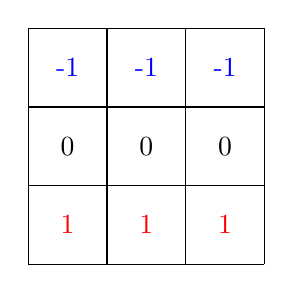
\begin{tikzpicture}
      % 垂直滤波器
  \draw (0,0) grid (3,3);
  
  \foreach \i/\j in {0/0, 1/0, 2/0}
    \node[red] at (\i+0.5, \j+0.5) {1};

    \foreach \i/\j in {0/1, 1/1, 2/1}
    \node at (\i+0.5, \j+0.5) {0};

    \foreach \i/\j in {0/2, 1/2, 2/2}
    \node[blue] at (\i+0.5, \j+0.5) {-1};

\end{tikzpicture}

\begin{equation}
    L_{content}\left(\vec{p},\vec{x},l\right)=\frac{1}{2} \sum_{i,j} \left(F_{ij}^l-P_{ij}^l\right)^2
\end{equation}

\begin{tikzpicture}
    % 垂直滤波器
\draw (0,0) grid (3,1);

\foreach \i in {3, 4, 5}
  \node at (\i+0.5, 0.5) {·};
  
  
\draw (6,0) grid (7,1);
\node at (6.5,0.5) {j};

\foreach \i in {7, 8, 9}
  \node at (\i+0.5, 0.5) {·};

\draw (10,0) grid (12,1);

\node at (6, -0.3) {$\underbrace{\hspace{12cm}}$};
\node at (6,-0.7) {原图中像素的个数};
\end{tikzpicture}

\begin{tikzpicture}
    % 垂直滤波器
\draw (0,0) grid (3,1);

\foreach \i in {3, 4, 5}
  \node at (\i+0.5, 0.5) {·};
  
  
\draw (6,0) grid (7,1);
\node at (6.5,0.5) {j};

\foreach \i in {7, 8, 9}
  \node at (\i+0.5, 0.5) {·};

\draw (10,0) grid (12,1);

\node at (6, -0.3) {$\underbrace{\hspace{12cm}}$};
\node at (6,-0.7) {特征图中像素的个数};
\end{tikzpicture}

\begin{tikzpicture}
	\draw (0,0) rectangle (10,10);
    \node at (5,5) {CNN} ;
\end{tikzpicture}


\end{document}
